\section{Empirical Verification}

\subsection{Linear model}

We want to see whether actual behavior of the models matches the behavior predicted from sensitivity analysis. By manually adjusting each crypt transition rate, we can identify the transition that has the greatest influence on cancer incidence. Figure 4 displays testing in the linear model. The red line representing $n_3 \rightarrow n_3$ is the most diverged from the black control line. Since sensitivity analysis predicts that changes to $n_3 \rightarrow n_3$ should cause the greatest shifts in the system, then this result is in agreement with the sensitivity analysis. This agreement is also statistically supported by the sum of squared error (SSE) analysis shown in Table 2. Biologically, it suggests that the degree to which APC-knockout crypts persist and multiply from year-to-year, is the most influential factor for cancer incidence, at least in this linear model using these specific parameter values.

\begin{figure}[h]
    \centering
    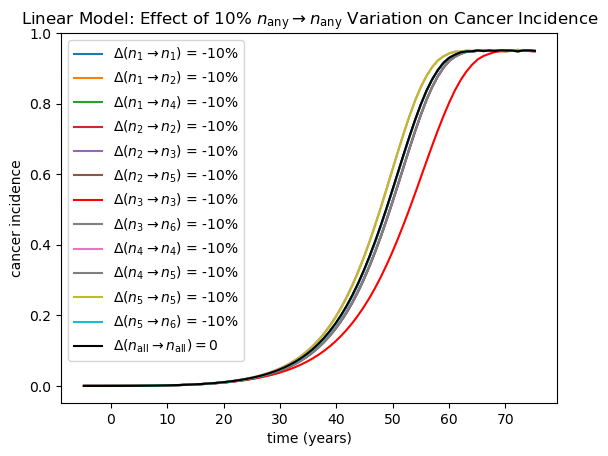
\includegraphics[width=0.65\linewidth]{figures/LinearEmpiricalPlot.png}
    \caption{Describes how a 10\% decrease in $n_i \rightarrow n_j$ affects cancer incidence in the linear model. The dotted black line represents the control case where $\Delta (n_{all} \rightarrow n_{all}) = 0$. Each colored line represents the cancer incidence when a 10\% decrease in each $n_{any} \rightarrow n_{any}$ is applied. Increased divergence from the black line suggests greater influence on cancer incidence. }
    \label{fig:linear sys empirical}
\end{figure}


\begin{table}[h]
  \centering
    \begin{tabular}{l|*{6}r}
    \toprule
    \multicolumn{7}{c}{SSE Associated with Varying Crypt Transition Rates in Linear ODE} \\
    \midrule
    \diagbox{Start}{End} & $n_1$ & $n_2$ & $n_3$ & $n_4$ & $n_5$ & $n_6$ \\
    \midrule
    $n_1$ &  $1.88E-2$ & $1.70E-2$  &   & $4.48 E -6$  &   &  \\ 
 $n_2$ &   & $1.71E-2$  & $1.58E-2$  &   & $3.01E-5$  &   \\ 
 $n_3$ &   &   & $\textcolor{red}{5.76E-1}$  &   &   & $1.58E-2$  \\ 
 $n_4$ &   &   &   & $4.29E-2$  & $4.85E-5$  &   \\ 
 $n_5$ &   &   &   &   & $3.97E-2$  &  $1.55E-4$ \\ 
 $n_6$ &   &   &   &   &   &   \\ 
    \bottomrule
    \end{tabular}%
  \caption{SSE is a quantitative measure of different between the black control line and each colored line in Figure 4. Larger SSE indicates a higher effect on cancer incidence. Any blank represents a transition that isn't relevant to this model. Red text marks the cell with highest SSE, indicating that this transition empirically has the greatest relative effect on cancer incidence.}
\label{tab:crypt_sse}
\end{table}

\subsection{Nonlinear model}
After verifying that  predicted and empirical behavior match in the linear model, we wanted to also verify this match or mismatch in the nonlinear model. Figure 5 displays testing in the nonlinear model. Multiple colored lines that mostly correspond to transitions between stages 3, 5, and 6 appear to be tied for furthest from the black line. In contrast to the fairly clean-cut results of the sensitivity analysis, this empirical testing doesn't suggest a single particular transition responsible for most of cancer incidence. This judgment is supported by the SSE values shown on table 3. These values describe $n_5 \rightarrow n_6$ as the most impactful crypt transition. The transition of interest $n_3 \rightarrow n_3$ barely trails behind in fourth place. This nonlinear system might be more resistant to changes compared to the linear approximation due to the carrying capacity term. Since the carrying capacity includes the sum $n_3 + n_4 + n_5$, it may be "coupling" the $n_3$, $n_4$, and $n_5$ transitions to each other, causing these transitions to behave similarly. Biologically, this result implies that crypt transitions from the last stages of precancer, stages 3 and 5, are broadly and similarly impactful on cancer incidence rates, at least in this nonlinear model using these specific parameter values.

\begin{figure}[h]
    \centering
    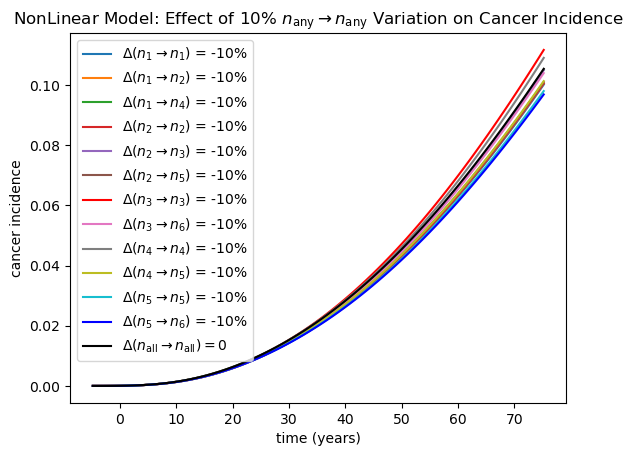
\includegraphics[width=0.65\linewidth]{figures/NonLinearEmpiricalPlot.png}
    \caption{Describes how a 10\% decrease in $n_i \rightarrow n_j$ affects cancer incidence in the nonlinear model. The dotted black line represents the control case where $\Delta (n_{all} \rightarrow n_{all}) = 0$. Each colored line represents the cancer incidence when a 10\% decrease in each $n_{any} \rightarrow n_{any}$ is applied.}
    \label{fig:nonlinear sys empirical}
\end{figure}

\begin{table}[h]
  \centering
    \begin{tabular}{l|*{6}r}
    \toprule
    \multicolumn{7}{c}{SSE Associated with Varying Crypt Transition Rates in NonLinear ODE} \\
    \midrule
    \diagbox{Start}{End} & $n_1$ & $n_2$ & $n_3$ & $n_4$ & $n_5$ & $n_6$ \\
    \midrule
    $n_1$ &  $5.22E-4$ & $4.11E-4$  &   & $4.48 E -6$  &   &  \\ 
 $n_2$ &   & $4.13E-4$  & $1.10 E -5$  &   & $2.98E-4$  &   \\ 
 $n_3$ &   &   & $4.95E-4$  &   &   & $5.22E-5$  \\ 
 $n_4$ &   &   &   & $1.35E-4$  & $2.823E-4$  &   \\ 
 $n_5$ &   &   &   &   & $9.03E-4$  &  $\textcolor{red}{1.17E-3}$ \\ 
 $n_6$ &   &   &   &   &   &   \\ 
    \bottomrule
    \end{tabular}%
  \caption{SSE is a quantitative measure of different between the black control line and each colored line in Figure 5. Larger SSE indicates a higher effect on cancer incidence. Any blank represents a transition that isn't relevant to this model. Red text marks the cell with highest SSE, indicating that this transition empirically has the greatest relative effect on cancer incidence.}
\label{tab:crypt_sse}
\end{table}